\documentclass[a4paper]{article}
\usepackage[english]{babel}
\usepackage[utf8x]{inputenc}
%\usepackage[T1]{fontenc}
\usepackage[letterpaper, margin=1in]{geometry} % page format
\usepackage{listings} % this package is for including code
\usepackage{graphicx} % this package is for including figures
\usepackage{amsmath}  % this package is for math and matrices
\usepackage{amsfonts} % this package is for math fonts
\usepackage{tikz} % for drawings
\usepackage{hyperref} % for urls
\usepackage{adjustbox}
\usepackage{pgfplots}
\usepackage{marvosym}

%%%%%%% Title %%%%%%%
\title{Final}
\author{Brian Henderson}
\date{12/11/17}
%%%%%%%%%%%%%%%%%%%%&

\pgfplotsset{compat=1.14}

\begin{document}
\maketitle

\section{Part 1}
Using the Mark dataset, vary the parameters to find which combination yields the best results by modifying the parameters of \texttt{lanmod.py}. Keep the \texttt{batch size} at 1, unless commenting out lines 351-352 in \texttt{lanmod.py}.

\subsection{Experiments Results}
\begin{table}[h]
 \caption{Experiments using different parameters to achieve lowest perplexity}
 \label{table}
 \begin{center}
 \resizebox{\textwidth}{!}{
  \begin{tabular}{lccccccccc||c}
    \hline \hline
     & Batch Size & Learning Rate & Layers & Steps & Hidden Size & Max Epoch & Max Max Epoch & Keep Prob & Decay & Perplexity \\
    \hline \hline
    0 & 1 & 1 & 2 & 20 & 200 & 4 & 13 & 1 & 0.5 & 1061.74 \\
    1 & 1 & 0.01 & 2 & 20 & 200 & 4 & 13 & 1 & 0.5 & 310.24 \\
    2 & 1 & 1 & 2 & 20 & 100 & 4 & 13 & 1 & 0.5 & 324.12 \\
    3 & 1 & 1 & 2 & 20 & 400 & 4 & 13 & 1 & 0.5 & 736.55 \\
    4 & 1 & 0.1 & 2 & 20 & 200 & 4 & 13 & 1 & 0.5 & 250.11 \\
    5 & 1 & 0.1 & 2 & 20 & 100 & 4 & 13 & 1 & 0.5 & 270.68 \\
    6 & 1 & 1 & 2 & 20 & 200 & 4 & 13 & 0.8 & 0.5 & 222.34 \\
    7 & 1 & 1 & 1 & 20 & 200 & 4 & 13 & 1 & 0.5 & 2030.20 \\
    \textbf{8} & \textbf{1} & \textbf{1} & \textbf{2} & \textbf{20} & \textbf{200} & \textbf{4} & \textbf{13} & \textbf{0.6} & \textbf{0.5} & \textbf{161.23} \\
    9 & 1 & 0.1 & 2 & 20 & 100 & 4 & 13 & 0.6 & 0.5 & 251.23 \\
    10 & 1 & 0.01 & 2 & 20 & 200 & 4 & 13 & 0.6 & 0.5 & 313.32 \\
    11 & 1 & 1 & 3 & 20 & 200 & 4 & 13 & 0.6 & 0.5 & 200.23 \\
    12 & 1 & 1 & 2 & 30 & 200 & 4 & 13 & 0.6 & 0.5 & 209.11 \\
    13 & 1 & 10 & 2 & 20 & 100 & 4 & 13 & 0.6 & 0.5 & 245.33 \\
    14 & 1 & 1 & 2 & 20 & 100 & 4 & 13 & 0.6 & 0.25 & 190.23 \\
    15 & 1 & 1 & 1 & 20 & 200 & 4 & 13 & 0.6 & 0.5 & 233.53 \\
    16 & 1 & 1 & 2 & 20 & 200 & 4 & 13 & 0.6 & 0.75 & 180.29 \\
    17 & 1 & 1 & 2 & 20 & 100 & 4 & 20 & 0.6 & 0.5 & 192.14 \\
    18 & 1 & 1 & 1 & 20 & 200 & 4 & 13 & 0.6 & 0.5 & 269.65 \\
    19 & 1 & 1 & 2 & 20 & 100 & 8 & 13 & 0.6 & 0.5 & 183.45 \\
    20 & 1 & 1 & 3 & 20 & 100 & 4 & 13 & 0.6 & 0.5 & 244.88 \\
    21 & 1 & 1 & 2 & 20 & 100 & 4 & 13 & 0.6 & 0.5 & 189.24 \\
    22 & 10 & 1 & 2 & 20 & 200 & 4 & 13 & 0.6 & 0.5 & 299.91 \\
    23 & 30 & 1 & 2 & 20 & 200 & 4 & 13 & 0.6 & 0.5 & 169.13  \\
    \hline \hline
  \end{tabular}}
 \end{center}
\end{table}

\subsection{Strategy of Experiments}
After reviewing the lab \textit{Language Modeling with RNNs/LSTMs} and researching which parameters were the most important to modify, I dove into the experiments. In order to get a base, I ran the architecture as it was originally set up, experiment \texttt{0}, to see where I was starting from and began modifying from their. For the majority of the experiments, the \texttt{Max Epoch} and \texttt{Max Max Epoch}, at the standard \texttt{4} and \texttt{13}, respectively. Based on the perplexity of the results of the combinations, I analyzed and made educated decisions on whether to continue to experiment with certain parameters of that combination. At the end, I played around with increasing the batch size, just to get an exposure to how that impacted the output of the architecture.

\subsection{Most Influential/Crucial/Important Parameters}
Based on the results, I found that the most important parameters were the learning rate and the keep probability. I found through certain experiments that the other parameters did not output as much of significant difference when modifying their values. There was a significant drop when modifying the keep probability from \texttt{1.0} to \texttt{0.6}. I also noticed that the \texttt{learning rate's} results varied highly on the other parameters. When modifying the \texttt{learning rate} in test 0 and 1, \texttt{learning rate 0.1} had a higher quality perplexity. However, when testing in experiments 8 and 9 using the \texttt{Keep Probability} of \texttt{0.6}, the \texttt{learning rate 1.0} had a higher quality testing perplexity.

\subsection{Least Influential/Crucial/Important Parameters}
Based on the results, I found that the lease influential parameters were the number of steps and hidden sizes as their output when modified to the various possible permutations was not as influential as the other parameters.

\subsection{Analyzing Experiment 08}
Experiment 08 had the lowest testing perplexity with a result of 161.23. For this architecture, the keep probability was the most influential parameter, as similar experiments with various keep probabilities had much higher perplexities.

\subsubsection{Training/Validation/Testing Perplexity Plot}
\begin{center}
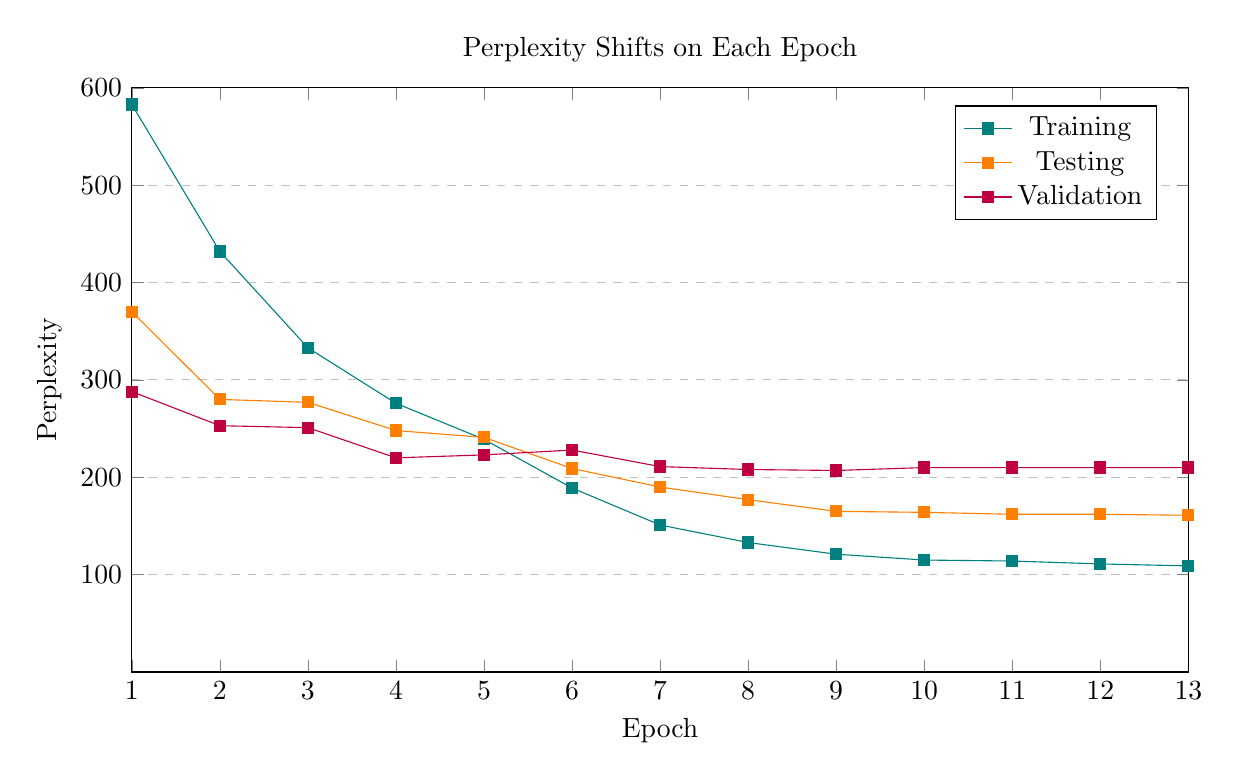
\begin{tikzpicture}
\begin{axis}[
    title={Perplexity Shifts on Each Epoch},
    xlabel={Epoch},
    ylabel={Perplexity},
    xmin=1, xmax=13,
    ymin=0, ymax=600,
    xtick={1,2,3,4,5,6,7,8,9,10,11,12,13},
    ytick={100, 200, 300, 400, 500, 600},
    legend pos=north east,
    ymajorgrids=true,
    grid style=dashed,
    height = 9cm,
    width = 15cm,
]
\addlegendentry{Training}
\addplot[
    color=teal,
    mark=square*,
    ]
    coordinates {
    (1,583) (2,432) (3,333) (4,276) (5,239) (6,189) (7,151) (8,133) (9,121) (10,115) (11,114) 	  (12, 111) (13, 109) 
    };
    
\addlegendentry{Testing}
\addplot[
    color=orange,
    mark=square*,
    ]
    coordinates {
 	(1,370) (2,280) (3,277) (4,248) (5,241) (6,209) (7,190) (8,177) (9,165) (10,164) (11,162) 	  (12,162) (13,161)
 	};

\addlegendentry{Validation}
\addplot[
    color=purple,
    mark=square*,
    ]
    coordinates {
 	(1,288) (2,253) (3,251) (4,220) (5,223) (6,228) (7,211) (8,208) (9,207) (10,210) (11,210) 	  (12,210) (13,210)
 	};


\end{axis}
\end{tikzpicture}
\end{center}

As seen by the graph above, the as the epochs continue to execute, the perplexity values from training, testing, and validation all had a similar trend, they started high and eventually evened out to their final perplexity values. This makes sense as the network trains itself to, \textit{in a good architecture}, be smarter and perform better. Keeping the perplexity values to a minimum is preferred for a smaller dataset. The  quality of the sentence that this architecture is poor compared to some other, even with a lower perplexity. For example, Experiment 08 produces this as the final sentence, \textit{"The crowd was the whole crowd was the whole crowd said to them, You are the Son of the Son of"}, which is very low quality. However, when executing Experiment 00, with a much higher perplexity, this was the final sentence, \textit{The priests and rolled marry the one of the council, who was also himself waiting expectantly for the kingdom of Man}. While this sentence is not exactly perfect english as well, it is still a much higher sentence quality. I would have expected that the quality of the sentence would have been in harmony with a lower testing perplexity, but this is not the case.

\subsection{Additional Thoughts}
After not seeing much of a decrease in the perplexity after many experiments, I began wondering why as this was definitely not the highest performance capable of achieving. I decided to take a look at the dataset. After exploring the dataset I noticed that in order to effectively run these experiments, I should have pre-processed the dataset so that identical words that were formatted differently, (lowercase vs uppercase first letters, punctuation, spaces), would all be the same in the vocabulary.

\section{Part 2}
I decided to take a quick look at how some of these experiments would run with a different dataset! Not much analysis was done on these problems, I simply did this to feed some curiosity that I have developed over this course. I used the best and worst set of parameters to run two experiments for the Trump Tweets data set

\subsection{Trump Tweets}
\subsubsection{Results}
\begin{table}[h]
 \caption{Experiments using Trump Tweets Data Set, Modifying the Keep Probability}
 \label{table}
 \begin{center}
 
  \begin{tabular}{c|c}
    \hline \hline
    Keep Prob & Perplexity \\
    \hline \hline
    1.0 & 802.41 \\
    0.6 & 863.28 \\
    \hline \hline
  \end{tabular}
 \end{center}
\end{table}

\subsubsection{Analysis}
 I ran these experiments using the default parameters and only modified the \texttt{keep probability} expecting to see as much of a difference as there was in the Mark data set. The Trump data set took quite a while to run, being that it is roughly 35,000 in size. Interesting enough, the final perplexity using this data set had opposite results. Using the Mark data set, the \texttt{keep probability} of \texttt{0.6} had a lower perplexity, but when using the Trump data set, it was higher. This shows the data set used has a huge influence on the parameters, and that the parameters should be tailored towards the data set. Unfortunately, I do not have enough time to explore this further, however, I will be conducting outside research to see how I can improve the sentence quality.

\subsubsection{Sentences Generated}
\textbf{Keep Prob 1.0:} "The attack which is a total joke and the U.S. is a total winner!I will be interviewed on @foxandfriends at"
\\\\
\textbf{Keep Prob 0.6:} "The Art of the U.S. and the great and the U.S. and the great and the U.S. and the great and"
\\\\\\
 Running these two experiments took over two hours on my gCloud instance (Tesla K80 GPU), leaving me without enough time to explore the PTB data set. \Frowny{}

\end{document}